\documentclass[10pt,answers]{exam}

\usepackage{mathtools}
\usepackage{amsmath}
\usepackage{amssymb}
\usepackage{xcolor}
\usepackage{soul}
\usepackage{graphicx}
\usepackage[top=2.0cm,bottom=2.0cm,left=2.5cm,right=2.5cm]{geometry}
\usepackage{tikz}
\usetikzlibrary{decorations.pathmorphing,patterns}
\usetikzlibrary {arrows.meta} 
\usepackage{float}
\usepackage{multicol}
\usepackage{pgfplots}
\usepackage{lastpage}
\usepackage{soul}
\usepackage{libertine}
\usepackage{lipsum}
\usepackage{siunitx}
\usepackage{xspace}
\usepackage[labelfont=bf]{caption}
\usepackage[hidelinks, urlcolor=blue, linkcolor=blue, citecolor=blue, colorlinks=true]{hyperref}
\usepackage[capitalize,noabbrev]{cleveref}
\usepackage[absolute]{textpos}

% code below allows to put more spaces between rows in bmatrix
\makeatletter
\renewcommand*\env@matrix[1][\arraystretch]{%
  \edef\arraystretch{#1}%
  \hskip -\arraycolsep
  \let\@ifnextchar\new@ifnextchar
  \array{*\c@MaxMatrixCols c}}
\makeatother

%========================================================================
% These are commands needed for the Markov chain example
%
\usepackage{tikz-network} % Required for drawing network diagrams for Markov chains
\usepackage{nicematrix} % Allows highlighting rows and columns of matrices
\usepackage[customcolors]{hf-tikz}

\usepackage{colortbl}

\tikzset{style blue/.style={
    set fill color=tolBlue!30,
    set border color = tolBlue!30
  },
  style orange/.style={
    set fill color=tolOrange!40,
    set border color = tolOrange!40
  },
  style red/.style={
    ,set fill color=tolRed!40,
    set border color = tolRed!40
  },
  style teal/.style={
    set fill color=tolTeal!40,
    set border color = tolTeal!40
  },
  style purple/.style={
    set fill color=tolPurple!40,
    set border color = tolPurple!40
  },
  style grey/.style={
    set fill color=tolGrey!40,
    set border color = tolGrey!40
  },
  hor/.style={
    above left offset={-0.1,0.31},
    below right offset={0.1,-0.125},
    #1
  },
  horshort/.style={
    above left offset={0.1,0.31},
    below right offset={-0.1,-0.125},
    #1
  },
  ver/.style={
    above left offset={-0.1,0.3},
    below right offset={0.1,-0.15},
    #1
  }
}
%========================================================================

\newcommand{\R}{ \mathbb{R}}
\newcommand{\C}{ \mathbb{C}}
\newcommand{\bA}{ \mathbf{A}}
\newcommand{\bp}{ \mathbf{p}}
\newcommand{\bx}{ \mathbf{x}}
\newcommand{\bz}{ \mathbf{0}}
% this gives me an open circle
\newcommand{\choice}{
\begin{tikzpicture}\draw (1,0) circle (1.0ex);\end{tikzpicture} \hspace{.1cm}}

% %correct choices in solution
\CorrectChoiceEmphasis{\rm}
\checkedchar{\tikz\draw[blue,fill=blue] (0,0) circle (1ex);}
\newcommand{\emptychoice}{
\begin{tikzpicture}\draw (1,0) circle (1.0ex);\end{tikzpicture}~~}
\newcommand{\fullchoice}{
\begin{tikzpicture}\draw[blue,fill=blue] (0,0) circle (1ex);\end{tikzpicture}~~}

\newcommand{\makeframednonemptybox}[3]{%
\setlength{\fboxrule}{0.5pt}
\fbox{%
\parbox[c][#1][t]{#2}{%
  \hrule width \hsize height 0pt%
  \vspace{\dimexpr(#1/2-0.1cm)}%
  \color{SolutionColor}#3\color{black}
 }%
}%
\setlength{\fboxrule}{1pt}
}

%% define course title
\newcommand{\course}{MAT185}
\newcommand{\assignmenttitle}{Assignment 4}

%% header and footer
\firstpageheader{}{}{\textbf{{\color{red} Due}: 10:00pm, Sunday Apr. 6, 2025}}
\firstpageheadrule
\runningheader{}{Page~\thepage~of~\numpages}{\course~--~\assignmenttitle}
\footer{}{}{}

\setlength\parindent{0pt} % no indentation in document

%% formats exam class
\qformat{\textbf{Question \thequestiontitle:}\hfill} % title of question 
\boxedpoints
\pointpoints{mark}{marks}
\pointsinrightmargin
\hpword{Marks:}
\hsword{Your score:}
\unframedsolutions
\totalformat{\boxed{\textnormal{\totalpoints~\if\totalpoints1 mark\else marks\fi}}}
\definecolor{SolutionColor}{rgb}{0,0,1}
\renewcommand{\solutiontitle}{}
\AtBeginEnvironment{solution}{\color{blue}}

% %correct choices in solution
\CorrectChoiceEmphasis{\rm}
\checkedchar{\tikz\draw[blue,fill=blue] (0,0) circle (1ex);}

% % increase distance between checkbox items
\renewcommand{\checkboxeshook}{\setlength{\itemsep}{6pt}}

%% distance between questions and parts
\renewcommand{\questionshook}{\setlength{\parsep}{10pt}}
\renewcommand{\partshook}{\setlength{\parsep}{15pt}}

%% define arrows in text
\newcommand{\arrow}{$\rightarrow$\xspace}
\newcommand{\Arrow}{$\Rightarrow$\xspace}

% % math notation:
%\veccol{1}{2}{3}{4}
\newcommand{\veccol}[4]{
    \begin{bmatrix}
      #1\\
      #2\\
      #3\\
      #4\\
    \end{bmatrix}}

\newcommand{\veccolTwo}[2]{
    \begin{bmatrix}
      #1\\
      #2\\
    \end{bmatrix}}

%%% This command makes a framed box of a chosen height.
\newcommand{\makenonemptybox}[2]{%
\par\nobreak\vspace{\ht\strutbox}\noindent
\setlength{\fboxrule}{0pt} % set this to 0pt to make invisible
\fbox{%
\parbox[c][#1][t]{\dimexpr\linewidth-2\fboxsep}{
  \hrule width \hsize height 0pt
  \vspace{-0.6cm}
  \color{SolutionColor}#2\color{black}
 }%
}%
\setlength{\fboxrule}{1pt}
}  
  
%\vecrow{1}{2}{3}
\newcommand{\vecrow}[3]{\left[#1~#2~ #3\right]}

%\matrixTwo{1}{2}{3}{4}
\newcommand{\matrixTwo}[4]{\left[\begin{array}{cc}#1&#2\\#3&#4\end{array}\right]}

% \matrixThree{1}{2}{3}{4}{5}{6}{7}{8}{9}
\newcommand{\matrixThree}[9]{\left[\begin{array}{ccc}#1&#2&#3\\#4&#5&#6\\#7&#8&#9\end{array}\right]}

%\matrixCorner{1}{2}{3}{4}
\newcommand{\matrixCorner}[4]{\left[\begin{array}{ccc}#1& \cdots&#2\\ \vdots & \ddots & \vdots\\#3&
      \cdots&#4\end{array}\right]}

% \nR
\newcommand{\nR}{{}^{n}\mathbb{R}}
% \Rn
\newcommand{\Rn}{\mathbb{R}^{n}}
% \nRn
\newcommand{\nRn}{{}^{n}\mathbb{R}^{n}}
% \nRm
\newcommand{\nRm}{{}^{n}\mathbb{R}^{m}}
% \nRm
\newcommand{\mRn}{{}^{m}\mathbb{R}^{n}}
% \mRm
\newcommand{\mRm}{{}^{m}\mathbb{R}^{m}}                              
       
%% define abbreviations
\newcommand{\row}{\operatorname{row}\,}
\newcommand{\col}{\operatorname{col}\,}
\renewcommand{\dim}{\operatorname{dim}\,}
\renewcommand{\span}{\operatorname{span}\,}
\newcommand{\rank}{\operatorname{rank}\,}
\renewcommand{\ker}{\operatorname{ker}\,}
\newcommand{\nul}{\operatorname{null}\,}
\renewcommand{\det}{\operatorname{det}\,}
\newcommand{\adj}{\operatorname{adj}\,}


\begin{document}

\vspace*{-0.5cm}
\begin{center}
  \large
  \textbf{\Large \course~--~Linear Algebra}\\[0.1cm]
  \textbf{\assignmenttitle}
\end{center}
\bigskip

\textbf{\large Instructions:}\\
\normalsize

Please read the {\bf MAT185 Assignment Policies \& FAQ} document for
details on submission policies, collaboration rules and academic integrity, and
general instructions.

\begin{enumerate}


\item \textbf{Submissions are only accepted by}
  \href{https://www.gradescope.ca}{Gradescope}. Do not send anything by email.
  Late submissions are not accepted under any circumstance. Remember you can
  resubmit anytime before the deadline.

\item \textbf{Submit solutions using only this template pdf}.  Your submission
  should be a single pdf with your full written solutions for each question. If
  your solution is not written using this template pdf (scanned print or
  digital) then your submission will not be assessed. Organize your work neatly
  in the space provided.  Do not submit rough work.

\item \textbf{Show your work and justify your steps} on every question but do
  not include extraneous information.  Put your final answer in the box
  provided, if necessary.  We recommend you write draft solutions on separate
  pages and afterwards write your polished solutions here on this template.

\item \textbf{You must fill out and sign the academic integrity statement
    below}; otherwise, you will receive zero for this assignment.

\end{enumerate}

\vspace{10pt}

\textbf{\large Academic Integrity Statement:} \\

%%% Student information

% Student 2
\fbox{
  \begin{minipage}{\textwidth}
    \vspace{0.75cm}
    \makebox[\textwidth]{\large Full Name: Siu, Nelson\enspace\hrulefill}\\[0.75cm]
    \makebox[\textwidth]{\large Student number: 1010940608\enspace\hrulefill}\\
  \end{minipage}
}
\vspace*{0.1in}

% Student 2
\fbox{
  \begin{minipage}{\textwidth}
    \vspace{0.75cm}
    \makebox[\textwidth]{\large Full Name: Cheung, Hei Shing\enspace\hrulefill}\\[0.75cm]
    \makebox[\textwidth]{\large Student number: 1010907823\enspace\hrulefill}\\
  \end{minipage}
}
\bigskip
\large \textbf{I confirm that:}
\normalsize

\begin{itemize} 
\item I have read and followed the policies described in the document {\bf
    MAT185 Assignment Policies \& FAQ}.
\item In particular, I have read and understand the rules for
  collaboration, and permitted resources on assignments as described in
  subsection II of the the aforementioned document. I have not violated
  these rules while completing and writing this assignment.
\item I have not used generative AI in writing this assignment.
\item I understand the consequences of violating the University's academic
  integrity policies as outlined in the
  \href{http://www.governingcouncil.utoronto.ca/policies/behaveac.htm}{Code of
    Behaviour on Academic Matters}. I have not violated them while completing
  and writing this assignment.
\end{itemize}
\bigskip

\large \textbf{By submitting this assignment to Gradescope, I agree that the
  statements above are true.}  \normalsize


\newpage

\section*{Preamble}

This assignment explores two applications for eigenvectors and eigenvalues:
(i) the PageRank algorithm and (ii) solving linear constant-coefficient second-order ordinary differential
equations.

\vspace{.2cm}

In Questions~\ref{question:PageRank} and \ref{question:PageRank2}, you will
explore using eigenvectors to calculate the ranking of nodes in a directed
graph, which is useful for ranking websites by how important they are, e.g., to
show a sorted list of websites based on a search criterion. The main problem
with ranking websites is that not every website is connected to every other
website.\footnote{A similar problem would be if you consider a tournament
  (e.g. a chess tournament), in which not every player is playing against every
  other player. How can we now calculate a ranking of the best players if we
  only have insufficient data?}  We are introducing a technique which is the
basis for the PageRank-algorithm, which is the main algorithm used by Google to
sort its search results in the 90s and is still in use today. Bryan and
Leise~\cite{Bryan2006} describe this algorithm in more detail and it is a great
insight if you are interested in more technical details. Reading this
publication is not necessary to solve the problems in this assignment. However,
we have uploaded
\href{https://q.utoronto.ca/courses/375036/modules/items/6183944}{the
  publication to Quercus} for the curious.

\vspace{.2cm}

In Question~\ref{question:ODE} we are using eigenvalues and eigenvectors to
solve an ordinary differential equation (ODE). In that case, we are using a
mass-spring system, representing other mechanics ODEs you will solve in the
following terms.

\subsection*{The PageRank Algorithm}
The PageRank algorithm is an important part of the internal functionality of web
search engines. It was established by Google and its founders Sergey Brin and
Larry Page in the 1990s. Its main functionality is based on their publication in
Reference~\cite{Brin1998}. We present here a key idea behind the PageRank
algorithm, which involves eigenvectors, eigenvalues, and directed graphs.  You
will work through a small example.  In reality, one needs to apply efficient
numerical algorithms to estimate the PageRank eigenvector.

\vspace{.2cm}

As an example, the directed graph in \cref{fig:graph1} represents a small
network of four websites. This graph has 4 \textit{nodes}, each representing a
website. If a website links to another website, this is shown by a directed
edge.  For example, website \#1 has two links: one to website \#2 and one to
website \#3.  Website \#2 also has two links: one to website \#3 and one to
website \#4.  We will only consider graphs for which every website links to some
other website and no website links to itself. (Although we encourage the curious
to explore such situations once they've worked through Question 1 and 2.)

\begin{figure}[H]
  \begin{center}
    \resizebox{0.25\textwidth}{0.25\textwidth}{
      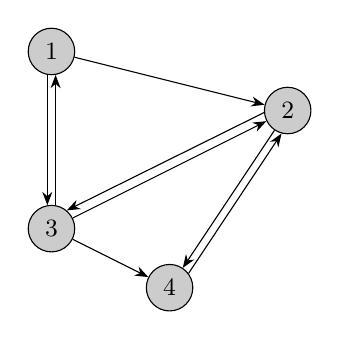
\begin{tikzpicture}[scale=0.75]
        \tikzstyle{every node}=[font=\small]
        \tikzset{vertex/.style = {shape=circle,draw,minimum size=0.5em}}
        \tikzset{edge/.style = {->,> = Stealth}}
        % vertices
        \node[vertex,fill={black!20}] (1) at  (0,1) {$1$};
        \node[vertex,fill={black!20}] (2) at  (4,0) {$2$};
        \node[vertex,fill={black!20}] (3) at  (0,-2) {$3$};
        \node[vertex,fill={black!20}] (4) at  (2,-3) {$4$};
        % edges
        \draw[edge] (1) to (2);
        \draw[edge] (2.185) to (3.50);
        \draw[edge] (1.260) to (3.100);
        \draw[edge] (3) to (2);
        \draw[edge] (2) to (4);
        \draw[edge] (3.80) to (1.280);
        \draw[edge] (3) to (4);
        \draw[edge] (4.37) to (2.255);
      \end{tikzpicture}}
  \end{center}
  \caption{Directed graph, representing a small network of linked websites.}
  \label{fig:graph1}
\end{figure}

One ranking strategy would be to use the number of incoming hyperlinks.  If lots
of other websites are linking to one website, surely that one website must be
very useful and reliable, right?  This strategy is flawed because it can be
easily manipulated by someone who creates lots of spurious websites all with
hyperlinks pointing to the one website they want to boost up in the ranking.
When creating a ranking, not all hyperlinks should carry the same weight!

\vspace{.2cm}

A hyperlink from a low-ranked website should have less of a contribution
to a website's ranking than a hyperlink from a high-ranked website.  Separately, there should
be some sort of dilution effect: if a website has two
hyperlinks pointing to other websites, those two links should count for more (on the receiving
ends) than if the website had ten hyperlinks pointing to other websites.

\newpage

The PageRank approach encapsulates these three ideas:
\begin{itemize}
\item The rank of a website is the sum of the weights of all incoming
  hyperlinks.
\item The higher the ranking of a website, the higher the weights are of its
  outgoing hyperlinks.
\item The more outgoing hyperlinks a website has, the lower the weight each of
  those hyperlinks has.
\end{itemize}
With this weighing strategy, we calculate the PageRank for each site as follows:
The PageRank $p_i$ of website $i$ is a positive scalar and is the weighted sum
of the PageRanks of all the websites that have hyperlinks pointing to it:
\begin{equation}
  \label{eq:1}
  p_i = \sum_{j\rightarrow i} \frac{p_j}{N_j}
\end{equation}
where $j \rightarrow i$ denotes there is a hyperlink from site $j$ to site $i$,
$p_j$ is the PageRank of website $j$, and $N_j$ is the total number of outgoing
hyperlinks from site $j$.  For example, to calculate the PageRank of website 2
in \cref{fig:graph1}, there is one incoming hyperlink from site 1 (which has 2
outgoing links), one from site 3 (which has 3 outgoing links), and one from site
4 (which has only one outgoing link). And so, the PageRank of $p_2$ is defined
as
\begin{equation}
  \label{eq:2}
  p_2 = \frac{1}{2} p_1 + \frac{1}{3} p_3 + p_4.
\end{equation}

In Question 1, you will find the PageRank of every website shown in
\cref{fig:graph1}.  In Question 2, you will continue studying the PageRank model
for this network and develop tools that will work for much, much larger
networks.

\vspace{.2cm}


\begin{thebibliography}{3}
\bibitem{Bryan2006} K. Bryan and T. Leise, \textit{The \$25,000,000,000
    Eigenvector: The Linear Algebra behind Google}, SIAM Review, 48:3, 569-581,
  2006,
  \href{https://q.utoronto.ca/courses/375036/modules/items/6183944}{[online]}.
\bibitem{Brin1998} S. Brin and L. Page, \textit{The anatomy of a large-scale
    hypertextual Web search engine}, Computer Networks and ISDN Systems, 30:1-7,
  107-117, 1998.
\end{thebibliography}

\newpage

\begin{questions}
  \question \label{question:PageRank}
  \begin{parts}
    \part \Cref{eq:2} determines the PageRank of node~2. Give the system of
    PageRank equations for the four nodes in \cref{fig:graph1}, as defined by
    \cref{eq:1}. \textit{No justification is required.}

    %%% Do not change the height of this box. Your work must fit inside it.
    \makenonemptybox{12em}{
      %%% Add your explanations here!      
      $$\begin{cases}
        p_1 &= \frac{1}{3}p_3 \\
        p_2 &= \frac{1}{2}p_1 + \frac{1}{3}p_3 + p_4 \\
        p_3 &= \frac{1}{2}p_1 + \frac{1}{2}p_2 \\
        p_4 &= \frac{1}{2}p_2 + \frac{1}{3}p_3 
      \end{cases}$$
      In matrix form, this is:
        $$\begin{bmatrix}
            0 & 0 & 1/3 & 0 \\
            1/2 & 0 & 1/3 & 1 \\
            1/2 & 1/2 & 0 & 0 \\
            0 & 1/2 & 1/3 & 0
            \end{bmatrix}
            \begin{bmatrix}
              p_1 \\ p_2 \\ p_3 \\ p_4
            \end{bmatrix}
            =
            \begin{bmatrix}
                p_1 \\ p_2 \\ p_3 \\ p_4
            \end{bmatrix}$$
      %%% end of your answer    
    }
    
    \part Formulate the linear system you found in part (a) as an
    eigenproblem. Identify the matrix $\mathbf{A}$, the eigenvalue and the
    eigenvector.  \label{part:q1_eigen}
        \textit{Note: you'll solve for the eigenvectors in the next part of this question.}

    %%% Do not change the height of this box. Your work must fit inside it.
    \makenonemptybox{15em}{
      %%% Add your explanations here!      
        For some eigenvector of $A$: $\mathbf{p} = \begin{bmatrix}
          p_1 & p_2 & p_3 & p_4
        \end{bmatrix}^T$, we can write the system of equations as
        $$A\mathbf{p} = \mathbf{p} = \begin{bmatrix}
            0 & 0 & 1/3 & 0 \\
            1/2 & 0 & 1/3 & 1 \\
            1/2 & 1/2 & 0 & 0 \\
            0 & 1/2 & 1/3 & 0
            \end{bmatrix}
            \begin{bmatrix}
              p_1 \\ p_2 \\ p_3 \\ p_4
            \end{bmatrix}
            =
            \lambda
            \begin{bmatrix}
              p_1 \\ p_2 \\ p_3 \\ p_4
            \end{bmatrix}$$
        where $\lambda = 1$. The matrix $\mathbf{A}$ is
        $$\mathbf{A} = \begin{bmatrix}
            0 & 0 & 1/3 & 0 \\
            1/2 & 0 & 1/3 & 1 \\
            1/2 & 1/2 & 0 & 0 \\
            0 & 1/2 & 1/3 & 0
            \end{bmatrix}$$
      %%% end of your answer    
    }
    
    \part \label{part:solve_eigen} Solve the eigenproblem you formulated in part
    (b).  Calculate the PageRank vector $\mathbf{p}$ for the graph in
    \cref{fig:graph1}.  You will need to use that the components of a PageRank
    vector must add up to 1.

    %%% Do not change the height of this box. Your work must fit inside it.
    \makenonemptybox{18em}{
      %%% Add your explanations here!
    Identifying $A\mathbf{p} = \mathbf{p}$ as an eigenvalue problem, we can
    solve for the eigenvector $\mathbf{p}$ by solving the system of equations $A\textbf{p} - \textbf{p} = 0$.
    This is equivalent to solving the system of equations $(A - I)\textbf{p} = 0$. So, we have:
    $$\begin{bmatrix}
        -1 & 0 & 1/3 & 0 \\
        1/2 & -1 & 1/3 & 1 \\
        1/2 & 1/2 & -1 & 0 \\
        0 & 1/2 & 1/3 & -1
        \end{bmatrix}
        \begin{bmatrix}
          p_1 \\ p_2 \\ p_3 \\ p_4
        \end{bmatrix}
        =
        \begin{bmatrix}
          0 \\ 0 \\ 0 \\ 0
        \end{bmatrix}$$
    We can solve this system of equations using computers method. I used the scipy.nullspace function in Python to find the null space of the matrix. The result is:
    $$\mathbf{p} = \text{span}\left(\begin{bmatrix}
        0.14547859 & 0.72739297 & 0.43643578 & 0.50917508       \end{bmatrix}^T\right)$$
    We can normalize this vector by dividing each component by the sum of all components:
    $$\sum_{i=1}^4 p_i = 0.14547859 + 0.72739297 + 0.43643578 + 0.50917508 = 1.81848242$$
    So, the PageRank vector is: 
    $$\mathbf{p} = \begin{bmatrix}
        0.14547859 & 0.72739297 & 0.43643578 & 0.50917508
      \end{bmatrix}^T/1.81848242 = \begin{bmatrix}
        0.08 & 
        0.4 & 
        0.24 & 
        0.28
        \end{bmatrix}^T$$
    }

    \newpage
    
    \part Which website of the graph in \cref{fig:graph1} has the highest and
    which has the lowest PageRank?
    
    %%% Do not change the height of this box. Your work must fit inside it.
    \makenonemptybox{10em}{
      %%% Add your explanations here!
      \begin{itemize}
        \item Website 2 has the highest PageRank of 0.4
        \item Website 1 has the lowest PageRank of 0.08
      \end{itemize}
      %%% end of your answer    
    }
    
    \part   
    Think about other possible networks.  What would be a network that would
    lead to all four webpages having the same PageRank?  Add the hyperlinks to
    the figure below on the left.  What would be a \textit{different} network
    would lead to all four webpages having the same PageRank? Add the hyperlinks
    to the figure on the right. \textit{No justification is required.}
    
    \textit{There are more than two possible answers to this question.  Please
      make sure that your hyperlinks are clearly legible in your scan, including
      the direction they're pointing.}
    
    \vspace{1cm}
    
    \begin{minipage}{.5\textwidth}
      \begin{center}
        \vspace{.3cm}
        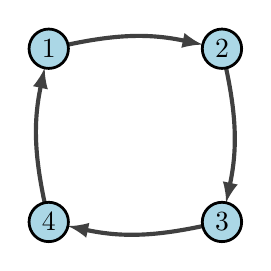
\begin{tikzpicture}[scale=.55]
          \Vertex[size = .5]{4} \Vertex[x=4,y=0, size = .5]{3}
          \Vertex[x=0,y=4,size = .5]{1} \Vertex[x=4,y=4, size = .5]{2}
          
          \draw (4) node {4};
          \draw (3) node {3};
          \draw (1) node {1};
          \draw (2) node {2};
           % % YOU CAN DRAW ARROWS WITH THE FOLLOWING COMMANDS
          \Edge[Direct,bend=12](1)(2)
            \Edge[Direct,bend=12](2)(3)
            \Edge[Direct,bend=12](3)(4)
            \Edge[Direct,bend=12](4)(1)

          % \Edge[Direct,loopshape=45,loopposition=0](2)(3)                        
        \end{tikzpicture}
        \end{center}
    \end{minipage}    
    %
 \begin{minipage}{.5\textwidth}
      \begin{center}
        \vspace{.3cm}
        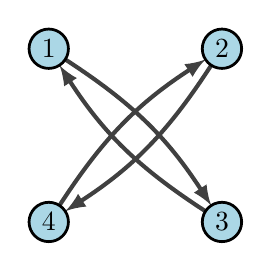
\begin{tikzpicture}[scale=.55]
          \Vertex[size = .5]{4} \Vertex[x=4,y=0, size = .5]{3}
          \Vertex[x=0,y=4,size = .5]{1} \Vertex[x=4,y=4, size = .5]{2}
          
          \draw (4) node {4};
          \draw (3) node {3};
          \draw (1) node {1};
          \draw (2) node {2};
           % % YOU CAN DRAW ARROWS WITH THE FOLLOWING COMMANDS
          % \Edge[Direct,bend=12](1)(2)
          \Edge[Direct,bend=12](1)(3)
            \Edge[Direct,bend=12](2)(4)
            \Edge[Direct,bend=12](3)(1)
            \Edge[Direct,bend=12](4)(2)
          % \Edge[Direct,loopshape=45,loopposition=0](2)(3)                        
        \end{tikzpicture}
        \end{center}
    \end{minipage}    
       
      
    \vspace{1.5cm}
    
  \end{parts}

\newpage

\question \label{question:PageRank2} Now that you are more familiar with the
eigenproblem from Question 1, you're going to study the eigenvalues and
eigenvectors of the matrix $\bA$ from Question 1.

\begin{parts}
  
  \part Compute $\bA \bx$ where $\bx \in {^4}\R$.  How is
  $\displaystyle\sum_{i=1}^4 (\bA \bx)_i$ related to
  $\displaystyle\sum_{i=1}^4 x_i$?\\[-1.0cm]

  %%% Do not change the height of this box. Your work must fit inside it.
  \makenonemptybox{11em}{
    \vspace{0.7cm}
    %%% Add your explanations here!
    %Since $A\mathbf{x} = \lambda \mathbf{x}$, we have $\sum_{i=1}^4 (\bA \bx)_i = \sum_{i=1}^4 \lambda x_i$. Which means:
    %$$\sum_{i=1}^4 (\bA \bx)_i = \sum_{i=1}^4 x_i$$
    %, since $\lambda = 1$.
    We consider the sum of the components of $\bA \bx$. First, we compute $\bA \bx$:
    $$\bA \bx = \begin{bmatrix}
        0 & 0 & 1/3 & 0 \\
        1/2 & 0 & 1/3 & 1 \\
        1/2 & 1/2 & 0 & 0 \\
        0 & 1/2 & 1/3 & 0
      \end{bmatrix}
      \begin{bmatrix}
        x_1 \\ x_2 \\ x_3 \\ x_4
      \end{bmatrix} =
      \begin{bmatrix}
        (1/3)x_3 \\ (1/2)x_1 + (1/3)x_3 + x_4 \\ (1/2)x_1 + (1/2)x_2 \\ (1/2)x_2 + (1/3)x_3
      \end{bmatrix}$$
    $$\sum_{i=1}^4 (\bA \bx)_i = (1/3)x_3 + (1/2)x_1 + (1/3)x_3 + x_4 + (1/2)x_1 + (1/2)x_2 + (1/2)x_2 + (1/3)x_3 = x_1 + x_2 + x_3 + x_4$$
      Thus, we have  $\sum_{i=1}^4 (\bA \bx)_i = \sum_{i=1}^4 x_i$


    %%% end of your answer    
  }

    
  Assume $\bx$ is an eigenvector of $\bA$ with eigenvalue $\lambda$.  What can
  you say about $\lambda$ and/or $\bx$?

  %%% Do not change the height of this box. Your work must fit inside it.
  \makenonemptybox{8em}{
    %%% Add your explanations here!
    Since $\bA \bx = \lambda \bx$, we can write: $\sum_{i=1}^4 (\bA \bx)_i = \sum_{i=1}^4 \lambda x_i$. 
    We know from the previous part that $\sum_{i=1}^4 (\bA \bx)_i = \sum_{i=1}^4 x_i$. So, we have $\sum_{i=1}^4 \lambda x_i = \sum_{i=1}^4 x_i$. 
    So, one of the following must be true:
    \begin{itemize}
      \item $\lambda = 1$ and $\bx$ is an eigenvector of $\bA$.
      \item $\sum_{i=1}^4 x_i = 0$ and $\lambda$ can be any value.
    \end{itemize}
    So, we can conclude that if $\bx$ is an eigenvector of $\bA$, then either
    $\lambda = 1$ or $\sum_{i=1}^4 x_i = 0$.
    %%% end of your answer    
  }

  
  \part Using your computation of $\bA \bx$ where $\bx \in {^4}\R$, how is
  $\displaystyle\sum_{i=1}^4 | (\bA \bx)_i |$ related to
  $\displaystyle\sum_{i=1}^4 |x_i|$?  \textit{You will want to use the triangle
    inequality: if $a, b \in \mathbb{R}$ then $|a+b| \leq |a| + |b|$.}

  %%% Do not change the height of this box. Your work must fit inside it.
  \makenonemptybox{11em}{
    %%% Add your explanations here!
    For all not necessarily eigenvectors $\bx \in {^4}\R$, we have:
    $
    (Ax)_i = \sum_{j=1}^4 A_{ij} x_j
    $
    Using the triangle inequality, we have:
    $$
    |(Ax)_i| = |\sum_{j=1}^4 A_{ij} x_j| \leq \sum_{j=1}^4 |A_{ij}| |x_j|
    $$
     \\Taking the sum over $i$ gives:
    $
    \sum_{i=1}^4 |(Ax)_i| \leq \sum_{i=1}^4 \sum_{j=1}^4 |A_{ij}| |x_j| = \sum_{j=1}^4 |x_j| \sum_{i=1}^4 |A_{ij}|
    $
    \\ Since $\sum_{i=1}^4 |A_{ij}| = 1$ for all $j$, we have:
    $$
    \sum_{i=1}^4 |(Ax)_i| \leq \sum_{j=1}^4 |x_j|
    $$
    
    %%% end of your answer    
  }

  If $\bx$ is an eigenvector of $\bA$, what can you say about its eigenvalue $\lambda$?

  %%% Do not change the height of this box. Your work must fit inside it.
  \makenonemptybox{8em}{
    %%% Add your explanations here!
    From the previous part, we know that $\sum_{i=1}^4 |(Ax)_i| \leq \sum_{j=1}^4 |x_j|$.
    Since $\bA \bx = \lambda \bx$, we have:
    $$
    \sum_{i=1}^4 |(Ax)_i| = |\lambda| \sum_{i=1}^4 |x_i| \leq \sum_{i=1}^4 |x_i|
    $$
    If $\bx$ is an eigenvector of $\bA$, be defintion we have $\sum_{i=1}^4 |x_i| \neq 0$. So, we can divide both sides by $\sum_{i=1}^4 |x_i|$:
    $$
    |\lambda| \leq 1
    $$
    
    %%% end of your answer    
  }

  \newpage
  
  \part Combining your answer to (a) and (b) what can you say about $\bA$'s
  eigenvalues and eigenvectors?

  %%% Do not change the height of this box. Your work must fit inside it.
  \makenonemptybox{3em}{
    %%% Add your explanations here!
    We have the following cases:
  \begin{itemize}
      \item If $\sum_{i=1}^4 x_i \neq 0$, then $|\lambda| = 1$.
      \item If $\sum_{i=1}^4 x_i = 0$, then $|\lambda| < 1$.
  \end{itemize}
  So, we can conclude that the eigenvalues of $\bA$ are all less than or equal to 1.
  %%% end of your answer    
  }
  
  \part Using matlab or python or wolframalpha or whatever, what are the
  eigenvalues of $\bA$?  Please give the eigenvalues in order of decreasing
  magnitude, largest to smallest.  Remember, $| a + i b | = \sqrt{a^2 + b^2}$.
  Round to two decimal places. \textit{No justification is required.}
  
  \begin{minipage}{.2\textwidth}
    $\lambda_1 \approx  $\makeframednonemptybox{0.5cm}{2cm}{1.00
    }
  \end{minipage}
  \hspace{.2cm}
  \begin{minipage}{.2\textwidth}
    $\lambda_2 \approx  $\makeframednonemptybox{0.5cm}{2cm}{-0.6 + 0.22i
    }
    [$|\lambda_2| \approx 0.64$]
  \end{minipage}
  \hspace{.2cm}
  \begin{minipage}{.2\textwidth}
    $\lambda_3 \approx  $\makeframednonemptybox{0.5cm}{2cm}{-0.6 - 0.22i
    }
    [$|\lambda_3| \approx 0.64$]
  \end{minipage}
  \hspace{.2cm}
  \begin{minipage}{.2\textwidth}
    $\lambda_4 \approx  $\makeframednonemptybox{0.5cm}{2cm}{0.20
    }
  \end{minipage}
  
  %% REPLACE \choice with \fullchoice FOR YOUR ANSWER
  Is $\bA \in {^4}\R^4$ diagonalizable? \hspace{.2cm}  \choice Yes \hspace{.4cm}  \fullchoice No
  
  %% REPLACE \choice with \fullchoice FOR YOUR ANSWER
  Is $\bA \in {^4}\C^4$ diagonalizable? \hspace{.2cm}  \fullchoice Yes \hspace{.4cm}  \choice No
  
  
  \part Let $\bx \in {^4}\C$ be a linear combination of the eigenvectors of $\bA$;
  that is, $\bx = c_1 \bx_1 + c_2 \bx_2 + c_3 \bx_3 + c_4 \bx_4$ where
  $c_i \in \C$.  What is $\bA \bx$?  What is $\bA^2 \,\bx$?  What is
  $\bA^{100} \,\bx$?  \textit{Your answers should include the symbols $\lambda_i$
    when referring to eigenvalues, rather than the approximate values you found
    for eigenvalues.}

  %%% Do not change the height of this box. Your work must fit inside it.
  \makenonemptybox{7em}{
    %%% Add your explanations here!
    Since $x_i$ are eigenvectors of $A$, we have:
    $$\bA \bx = c_1 \lambda_1 \bx_1 + c_2 \lambda_2 \bx_2 + c_3 \lambda_3 \bx_3 + c_4 \lambda_4 \bx_4$$
    Since $\bA$ is a linear operator, $\bA(c_1 \bx_1 + c_2 \bx_2 + c_3 \bx_3 + c_4 \bx_4) = c_1 \bA \bx_1 + c_2 \bA \bx_2 + c_3 \bA \bx_3 + c_4 \bA \bx_4$ and we can write:
    $$\bA^2 \bx = c_1 \lambda_1^2 \bx_1 + c_2 \lambda_2^2 \bx_2 + c_3 \lambda_3^2 \bx_3 + c_4 \lambda_4^2 \bx_4$$
    $$\bA^{100} \bx = c_1 \lambda_1^{100} \bx_1 + c_2 \lambda_2^{100} \bx_2 + c_3 \lambda_3^{100} \bx_3 + c_4 \lambda_4^{100} \bx_4$$
    %%% end of your answer    
  }
  
  As $n \to \infty$, what does $\bA^n \, \bx$ do, and why?
  
  %%% Do not change the height of this box. Your work must fit inside it.
  \makenonemptybox{3em}{
    %%% Add your explanations here!
    Since $|\lambda_1| = 1$ and $|\lambda_2|, |\lambda_3|, |\lambda_4| < 1$, we have:
    $$\bA^n \bx = c_1 \lambda_1^n \bx_1 + c_2 \lambda_2^n \bx_2 + c_3 \lambda_3^n \bx_3 + c_4 \lambda_4^n \bx_4$$
    As $n \to \infty$, the terms with $\lambda_2$, $\lambda_3$ and $\lambda_4$ will go to 0, and we will be left with $\bA^n \bx \to c_1 \bx_1$.
    %%% end of your answer    
  }
  
  \part You have the matrix $\bA$ and you would like to find an approximation of
  an eigenvector for the eigenvalue $1$.  You have access to matlab and python but
  not to subroutines that compute eigenvalues and eigenvectors.
  Playing around, you discover that if you choose a random vector $\bx \in {^4}\R$
  and you compute $\bA^n \, \bx$ for larger and larger values of $n$ then
  $\bA^n \, \bx$ seems to stop changing (so far as the computer can see).  If you
  call that computational limit $\bx_\infty$, is $\bx_\infty$ (approximately) an
  eigenvector for $\bA$ with eigenvalue $1$?

  %% REPLACE \choice with \fullchoice FOR YOUR ANSWER
  \hspace{.2cm}  \choice Yes \hspace{.4cm}  \fullchoice No  
  
  If yes, why?  If no, why not?
  %%% Do not change the height of this box. Your work must fit inside it.
  \makenonemptybox{4em}{
    %%% Add your explanations here!
    No, since $x_\infty$ is the image of the random vector $\bx$ under the
    transformation $\bA^n$, it is not guaranteed that $\bx$ not be spanned only by $\bx_2, \bx_3$ and $\bx_4$. 
    If $c_1 = 0$, then $\bA^n \bx_\infty$ will not converge to an eigenvector of $\bA$ and converge to the zero vector.
    For instance, we pick $\bx = \bx_3$, then $\bA^n \bx_\infty = c_3 \lambda_3^n \bx_3$ and as $n \to \infty$, $\bA^n \bx_\infty$ will converge to 0.
    So, we can conclude that $\bx_\infty$ is not guaranteed to converge to the eigenvector of $\bA$ assocated with the eigenvalue 1.
    %%% end of your answer    
  }
  
\end{parts}


\begin{EnvUplevel}  
  \textit{\textbf{For the curious:}} The linear system in question 1(a) is a
  small linear system: four equations in four unknowns.  Your immediate reaction
  upon seeing the system should have been to set up an augmented matrix, do some
  elementary row operations, and find all solutions.  Finding solutions by
  viewing it as an eigenproblem seems pretty artificial!  And even if you do
  decide to take the eigenproblem view of things; you can find the null space of
  $ \mathbf{I} - A$ via row reduction.  So row reduction must be the right
  approach, right?
   
  For a internet search engine, how big is the matrix $\mathbf{A}$?  Its size
  depends on the number of considered webpages, which is roughly on the order of
  tens of billions for a search engine.  We do know that the $\textbf{A}$ is
  very sparse because, on average, there are fewer than 100 links per webpage
  pointing to different page. So, $\bA$ is a sparse matrix of size 10 billion
  $\times$ 10 billion. The number of operations needed to transform an
  $n \times n$ matrix to reduced row echelon form is $\mathcal{O}(n^3)$.  But
  the number of operations needed to compute $\bA \bx$ once is
  $\mathcal{O}(n^2)$.  When you have $\bA \bx$, computing $\bA^2 \bx$ is a
  matter of computing $\bA (\bA \bx)$ --- this will be another
  $\mathcal{O}(n^2)$.  Computing $\bA^k \, \bx$ is $\mathcal{O}(k n^2)$ and so,
  if $k$ isn't large, this will be faster than computing the reduced row echelon
  form.  Using this approach to approximate an eigenvector for the largest
  eigenvalue is called \textit{power method}.  It works well as long as the
  geometric multiplicity of the largest eigenvalue is 1.  The speed with which
  it converges has to do with how big the gap is between $|\lambda_1|$ and
  $|\lambda_2|$ where $\lambda_2$ is an eigenvalue with ``next largest" size.
  The bigger $|\lambda_1| - |\lambda_2|$ is, the faster the power method
  converges.  You can find Python implementations of the power method to
  calculate the dominant eigenvalue and eigenvector
  \href{https://www.geeksforgeeks.org/power-method-determine-largest-eigenvalue-and-eigenvector-in-python/}{online}.
    
  Numerical methods for computing eigenvalues have been an area of active
  research and continue to be so.  The power method is a snowflake on top of an
  iceberg when it comes to the topic!
    
  A separate question is: what properties of a network ensure that $1$ will be
  an eigenvalue of the matrix $\bA$?  What properties ensure that its eigenspace
  will be one dimensional?

\end{EnvUplevel}
  
\newpage 
     
\question \label{question:ODE} The typical ODEs in mechanics are second-order
ODEs, because the acceleration is the second derivative of the position in
respect to time. If the ODEs are linear, they can be reformulated as two linear
first-order ODEs.  If the ODEs have constant coefficients and if the forcing is
constant, we can solve the system using the methods from this course.
  
In this problem, you will will explore solving a second-order ODE which
describes a mass-spring system using the techniques discussed in this course.
\textit{For the curious: the methods used in this problem work equally well if
  there is damping in the system and these methods apply for other oscillatory
  systems such as RL circuits and RLC circuits.}

Consider the following mass-spring system with one mass and two springs:
\bigskip
  
\begin{figure}[H]
  \begin{center}
    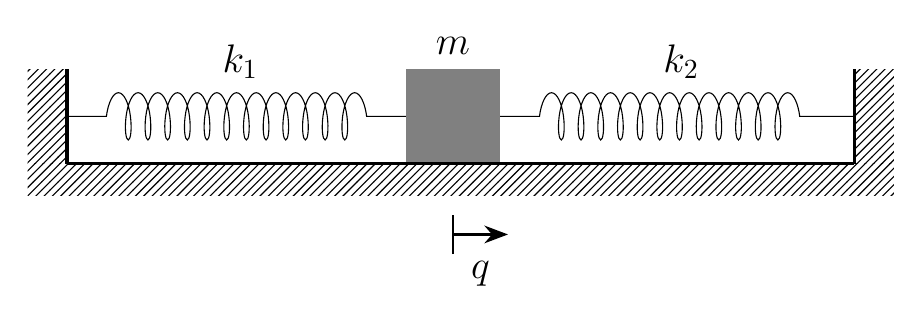
\begin{tikzpicture}
      \draw[decoration={aspect=0.3, pre length=0.5cm,post length=1.0cm, segment
        length=2.5mm, amplitude=3mm,coil},decorate] (-5,0) -- (0,0);
      \draw[decoration={aspect=0.3, pre length=1.0cm,post length=0.5cm, segment
        length=2.5mm,amplitude=3mm,coil},decorate] (0,0) -- (5,0);
      \node[rectangle,fill=gray,inner sep=6mm] (a) at (-0.1,0) {};
      \fill [pattern = north east lines] (-5.5,-0.6) rectangle (-5,0.6);
      \draw[very thick]
      (-5,-0.6) -- (-5,0.6);
      \fill [pattern = north east lines] (5.5,-0.6) rectangle (5,0.6); \draw[very thick]
      (5,-0.6) -- (5,0.6);
      \fill [pattern = north east lines] (-5.5,-0.6) rectangle (5.5,-1.0);
      \draw[very thick] (-5,-0.6) -- (5,-0.6);
      \node[] at (-0.1,0.9) {\Large $m$};
      \node[] at (-2.8,0.7) {\Large $k_1$};
      \node[] at (2.8,0.7) {\Large $k_2$};
      \draw[-{Stealth[length=3mm]},thick] (-0.1,-1.5) -- (0.6,-1.5);
      \draw[thick] (-0.1,-1.75) -- (-0.1,-1.25);
      \node[] at (0.25,-2.0) {\Large $q$};
    \end{tikzpicture}
  \end{center}
  \caption{Mass-spring system with the mass $m$ and two springs of
    stiffness $k_1$ and $k_2$.}
  \label{fig:mass_spring}
\end{figure}
We will ignore the effect of gravity and of friction and we will assume the
displacements are small enough that Hooke's law applies.  Let $m$ be the mass,
and $k_1$ and $k_2$ be the spring constants (i.e. the stiffnesses) of the
springs. The equation of motion for the system in \cref{fig:mass_spring} is
\begin{equation}
  \label{eq:ode}
  m \ddot{q}(t) = -k_1 q(t) - k_2 q(t)  = -(k_1 + k_2)q(t).
\end{equation}
Here, $q$ is the displacement from rest; if the system is at rest then
$q(t)=0$ for all time $t$.  To understand the force: a displacement of the
mass $m$ in positive $q$ direction result in the left spring to lengthen,
which leads to pulling in $-q$ direction, and the right spring to compress,
which leads to pushing in $-q$ direction.
  
  \begin{parts}
    
    \part Using the substitution of $x_1(t) = q(t)$ and $x_2(t) = \dot q(t)$, show
 that  
    \cref{eq:ode}  can
    be expressed as the following system of two first-order ODEs:
    \begin{equation}
      \label{eq:subst}
      \dot{\mathbf{x}}(t)=\veccolTwo{\dot{x}_1(t)}{\dot{x}_2(t)}=\matrixTwo{0}{1}{-\frac{k_1+k_2}{m}}{0}\veccolTwo{x_1(t)}{x_2(t)}=\mathbf{A}\mathbf{x}(t).
    \end{equation}

    %%% Do not change the height of this box. Your work must fit inside it.
    \makenonemptybox{10em}{
      %%% Add your explanations here!
      From \cref{eq:ode}, we have:
       $$m \dot{x}(t) = m \ddot{q}(t) = -k_1 q(t) - k_2 q(t)  = -(k_1 + k_2)q(t) = -k q(t)$$
      So, we have:
        $$\dot{x}(t) = -\frac{k_1 + k_2}{m} x(t) \cdot (1)$$
      Also, we have the definition of $x_1$ and $x_2$: $x_1(t) = q(t)$ and $x_2(t) = \dot{q}(t)$, so we can write:
    $$\dot{x}_1(t) = \dot{q}(t) = x_2(t)$$ 
    Constructing the system of equations, we have:
    $$\begin{bmatrix}
        0 & 1 \\
        -\frac{k_1 + k_2}{m} & 0
        \end{bmatrix} \begin{bmatrix}
        x_1(t) \\
        x_2(t)
        \end{bmatrix} = \begin{bmatrix}
        \dot{x}_1(t) \\
        \dot{x}_2(t)
        \end{bmatrix}$$


       %%% end of your answer    
    }
  \newpage

  \begin{EnvUplevel}
    You will now solve \cref{eq:ode}, using \cref{eq:subst} and
    the methods introduced in this course.
  \end{EnvUplevel}

  \part \label{part:eigenvalue} View $\bA$ as a complex matrix, rather than a
  real one, $\bA \in {^2}\C^2$, and compute the eigenvalues of $\mathbf{A}$ from
  \cref{eq:subst}.  To keep your computations simple, replace $k_1+k_2$ with $k$
  (the effective spring constant).  Your eigenvalues should be of the form
  $\pm i \omega$ where $\omega$ is a function of $k$ and $m$.  The expression you will find for $\omega$ is called the
  ``natural angular frequency'' or the ``natural frequency''.  For the rest of
  Question 3, refer to $\omega$ rather than to expressions involving $k$ and
  $m$.

  %%% Do not change the height of this box. Your work must fit inside it.
  \makenonemptybox{25em}{
    %%% Add your explanations here!
    The eigenvalues of $A$ are the solutions of the characteristic polynomial:
    $$\det(A - \lambda I) = 0$$
    We have:
    $$A - \lambda I = \begin{bmatrix}
        0 & 1 \\
        -\frac{k}{m} & 0
      \end{bmatrix} - \begin{bmatrix}
        \lambda & 0 \\
        0 & \lambda
      \end{bmatrix} = \begin{bmatrix}
        -\lambda & 1 \\
        -\frac{k}{m} & -\lambda
      \end{bmatrix}$$
    So, we have:
    $$\det(A - \lambda I) = \det \begin{bmatrix}
        -\lambda & 1 \\
        -\frac{k}{m} & -\lambda
      \end{bmatrix} = (-\lambda)(-\lambda) - (1)(-\frac{k}{m}) = \lambda^2 + \frac{k_1 + k_2}{m}$$
    Setting the determinant to 0, we have:
    $$\lambda^2 + \frac{k}{m} = 0$$
    $$\lambda^2 = -\frac{k}{m}$$
    $$\lambda = \pm i \sqrt{\frac{k}{m}}$$
    Setting $\omega = \sqrt{\frac{k}{m}}$, we have:
    $$\lambda = \pm i \omega$$
    %%% end of your answer    
  }

  \part \label{part:e_vec} Compute the eigenvectors for the two complex
  eigenvalues calculated in
  Question~\ref{question:ODE}\,(\ref{part:eigenvalue}). \textit{\textbf{Hint:}}
  The eigenvectors will be complex as well.  \textit{You will need to rewrite
    $\bA$ so that it no longer involves $k$ and $m$, only $\omega$.}

  %%% Do not change the height of this box. Your work must fit inside it.
  \makenonemptybox{20em}{
    %%% Add your explanations here!
    We consider the matrix:
    $$A \pm i \omega I = \begin{bmatrix}
        0 & 1 \\
        -\omega^2 & 0
      \end{bmatrix} \pm i \begin{bmatrix}
        \omega & 0 \\
        0 & \omega
        \end{bmatrix} = \begin{bmatrix}
        \pm i \omega & 1 \\
        -\omega^2 & \pm i \omega
      \end{bmatrix}$$
    %%% end of your answer  
    Considering the first eigenvalue $\lambda_1 = i \omega$, and consider any $c_1, c_2 \in \C$, we have:
    $$\begin{bmatrix}
        i \omega & 1 \\
        -\omega^2 & i \omega
      \end{bmatrix} \begin{bmatrix}
        x_1 \\
        x_2
      \end{bmatrix} = 0$$
    So the first eigenvector is $c_2[1, i \omega]^T$. Considering the second eigenvalue $\lambda_2 = -i \omega$, we have:
    $$\begin{bmatrix}
        -i \omega & 1 \\
        -\omega^2 & -i \omega
      \end{bmatrix} \begin{bmatrix}
        x_1 \\
        x_2
      \end{bmatrix} = 0$$
    So the second eigenvector is $c_2[1, -i \omega]^T$.  So the eigenvectors are:
    $$c_1\begin{bmatrix}
        1 \\
        i \omega
      \end{bmatrix} \text{ and } c_2\begin{bmatrix}
        1 \\
        -i \omega
      \end{bmatrix}$$
  }
  
  \newpage
  
  \part Using the eigenvalues and eigenvectors you found, what is the general
  solution, $\bx(t)$, for the system in \cref{eq:subst}?  What is each component, $x_1(t)$ and
  $x_2(t)$?  \textit{Please keep working with $\omega$ rather than $k$ and $m$.
    Also, you want to check your work by checking on a piece of scratch paper that $\dot{x}_1(t) = x_2(t)$.  There's no need to present that verification here.}

  %%% Do not change the height of this box. Your work must fit inside it.
  \makenonemptybox{6em}{
       Given $\lambda_1 = i \omega$ and $\lambda_2 = -i \omega$, we have:
    $$\begin{bmatrix}
        x_1(t) \\
        x_2(t)
      \end{bmatrix} = c_1 e^{i \omega t} \begin{bmatrix}
        1 \\
        i \omega
        \end{bmatrix} + c_2 e^{-i \omega t} \begin{bmatrix}
        1 \\
        -i \omega
        \end{bmatrix}$$
    So, we have:
    $$x_1(t) = c_1 e^{i \omega t} + c_2 e^{-i \omega t}$$
    $$x_2(t) = c_1 i \omega e^{i \omega t} - c_2 i \omega e^{-i \omega t} = i \omega (c_1 e^{i \omega t} - c_2 e^{-i \omega t})$$
    
  }
    
  \part Assume that the mass is initially at rest, $q(0)=q_0$ and
  $\dot{q}(0) = 0$.  This determines $\bx(0)$.  What is $\bx(t)$?
 \textit{At this
    point, we haven't discussed what it means to have a complex number in the
    exponent but you do still know that $e^0=1$.}

  %%% Do not change the height of this box. Your work must fit inside it.
  \makenonemptybox{8em}{
    %%% Add your explanations here!
    First, we solve for $c_1$ and $c_2$ using the given initial conditions:
    $$x_1(0) = c_1 = c_2 = q_0 \quad x_2(0) = i \omega (c_1 - c_2) = \dot{q}(0) = 0$$
    Thus, by sovling the system of equations, we have $c_1 + c_2 = q_0/2$. Therefore, we have:
    $$\bx = \begin{bmatrix}
        x_1(t) \\
        x_2(t)
      \end{bmatrix} = \begin{bmatrix}
        c_1 e^{i \omega t} + c_2 e^{-i \omega t} \\
        i \omega (c_1 e^{i \omega t} - c_2 e^{-i \omega t})
      \end{bmatrix} = \begin{bmatrix}
        \frac{q_0}{2} e^{i \omega t} + \frac{q_0}{2} e^{-i \omega t} \\
        i \omega (\frac{q_0}{2} e^{i \omega t} - \frac{q_0}{2} e^{-i \omega t})
      \end{bmatrix}$$
    %%% end of your answer    
  }
  
  \part At this point, you have an expression for $q(t)$ that involves $i$.  Use
  Euler's formula, $e^{i\theta} =\cos \theta + i \sin \theta$, to express $q(t)$
  in terms of real quantities only.  \textit{\textbf{For the curious:} you can
    use these ideas to rewrite the general solution from part (d) as something
    involving $\cos$ and $\sin$ if you assume the initial conditions
    $q(0) = q_0$ and $\dot{q}(0) = v_0$.}

  %%% Do not change the height of this box. Your work must fit inside it.
  \makenonemptybox{18em}{
    %%% Add your explanations here!
    Using the results of the initial conditions, using Euler's formula, we can rewrite $q(t)$ as:
    $$q(t) = \frac{q_0}{2} e^{i \omega t} + \frac{q_0}{2} e^{-i \omega t} = \frac{q_0}{2} (\cos(\omega t) + i \sin(\omega t)) + \frac{q_0}{2} (\cos(-\omega t) + i \sin(-\omega t))$$
    $$= \frac{q_0}{2} (\cos(\omega t) + i \sin(\omega t)) + \frac{q_0}{2} (\cos(\omega t) - i \sin(\omega t))$$
    The imaginary parts cancel out, so we have:
    $$q(t) = \frac{q_0}{2} (\cos(\omega t) + \cos(\omega t)) = q_0 \cos(\omega t)$$
    So, we have:
    $$q(t) = q_0 \cos(\omega t)$$
    %%% end of your answer    
  }


  \part Check if your found solution for $q(t)$ satisfies the ODE in
  \cref{eq:ode}.

  %%% Do not change the height of this box. Your work must fit inside it.
  \makenonemptybox{3em}{
    %%% Add your explanations here!
    $$ \ddot{q}(t) = -\omega^2 q(t)$$
    $$m \ddot{q}(t) = -k_1 q(t) - k_2 q(t) = -(k_1 + k_2)q(t)$$
    %%% end of your answer    
  }
  
\end{parts}

\end{questions}

\end{document}
